\chapter{Introduction}\label{ch:introduction}

\section{The Sub-Neptune Population and the Characterization Crisis}

Sub-Neptune exoplanets represent the most abundant planetary demographic in the Milky Way
\cite{fulton2017}, yet they remain profoundly misunderstood. Defined as planets with radii
between Earth ($1\,R_\oplus$) and Neptune ($\approx 4\,R_\oplus$) and masses of
4--10\,$M_\oplus$ \cite{fulton2017}, sub-Neptunes are ubiquitously discovered by transit
surveys, including Kepler and TESS. Their frequency alone, surpassing both terrestrial
super-Earths and gas giants by a factor of two to three \cite{petigura2018}, demands that
planetary science develop a coherent theoretical framework for understanding their formation,
composition, and evolution.

Observational constraints reveal that sub-Neptunes possess a complex internal architecture:
rocky or icy cores enveloped by thick, voluminous atmospheres dominated by hydrogen and helium
(approximately 75\% H and 25\% He by mass \cite{madhusudhan2025}). This composition places
them in a transitional regime between rocky terrestrial planets and gas giants, a structural
uniqueness that has no direct analogue in our solar system. This absence of a solar system
template proves deeply problematic. We cannot simply scale the physics of terrestrial planet
outgassing or giant planet formation to understand sub-Neptunes; their formation and
evolutionary pathways must have diverged fundamentally from those of familiar planetary
types.

Yet, despite decades of exoplanet discoveries and recent breakthroughs in atmospheric
characterization via JWST, fundamental properties remain poorly constrained: the total
volatile inventory, the internal redox state of the mantle, the thermal structure at depth,
and critically, the composition and long-term stability of the magma ocean boundary.

\section{The Magma Ocean Problem: Why Coupled Modeling Matters}

The defining geophysical feature of young sub-Neptunes is the presence of a \textbf{magma
ocean}, a region of extensive silicate melting at the top of the planetary mantle, above the
core of the planet and directly underlying the volatile-rich atmosphere.

Considerable evidence supports this scenario. The high internal temperatures of
sub-Neptunes, maintained by accretionary heating during rapid formation and the insulating
effect of their thick H/He envelopes, naturally lead to mantle temperatures exceeding the
silicate liquidus at relevant pressures. Magma oceans persist for extended periods,
potentially millions of years, as the planet gradually cools and the mantle crystallizes
\cite{hamano2013}. During this prolonged molten phase, the magma-atmosphere boundary becomes
an extraordinarily active chemical interface, not a passive boundary.

Yet the magma ocean problem reveals a critical gap in our theoretical framework. Classical
atmosphere models treat the overlying gas as chemically decoupled from the interior,
calculating equilibrium compositions as if the atmosphere were isolated from mantle
processes. This approach is demonstrably incorrect for sub-Neptunes. In our bachelor thesis
\cite{laga2025} we showed with \Atm{} that the magma ocean acts as a dominant control on
atmospheric state: a redox-dependent solubility pump stores hydrogen as dissolved water, and
the atmospheric CO$_2$/CH$_4$ ratio traces the oxidation state of the mantle.

First-principles simulations have since sharpened this picture. Gilmore \& Stixrude
\cite{gilmore2026} showed with density-functional-theory molecular dynamics (DFT-MD) that
hydrogen and MgSiO$_3$ liquid are \textbf{completely miscible} above a critical temperature
$T_C$ that decreases from about 3,500\,K at 2\,GPa to 2,600\,K at 10\,GPa. The conditions
at the magma-atmosphere boundary of most sub-Neptunes lie above this critical curve for much
of their early evolution \cite{gilmore2026,young2025}. The interior and the envelope are then
one fluid, rather than a melt in contact with a gas. As the planet cools, the interior
crosses the coexistence curve (the \textbf{binodal}) and hydrogen exsolves into the envelope
\cite{rogers2025,rogers2026,tejada2026}. This is the exsolution of incompatible volatiles
during cooling that our thesis identified as a possible cause of late-stage atmospheric
inflation \cite{laga2025}.

\section{Spinodal Decomposition and Delayed Exsolution}\label{sec:spinodal_intro}

Current evolution models assume that hydrogen exsolves as soon as the bulk composition
enters the miscibility gap, that is, at the binodal \cite{rogers2025,rogers2026}. A
homogeneous mixture just inside the binodal, however, is \emph{metastable} rather than
unstable. Forming the new phase requires nucleation, which has to overcome a free-energy
barrier \cite{debenedetti1996,kashchiev2000}. Only at the \textbf{spinodal}, where the
curvature of the Gibbs free energy with respect to composition vanishes, does the mixture
become unstable to small composition fluctuations and decompose spontaneously. This process
is \textbf{spinodal decomposition} \cite{cahn1958,cahn1961}. Between the binodal and the
spinodal lies a metastable window (Figure~\ref{fig:concept}). If nucleation is suppressed,
exsolution is delayed until the spinodal. If nucleation is easy, for example on existing
interfaces, the delay vanishes.

\begin{figure*}[t]
\centering
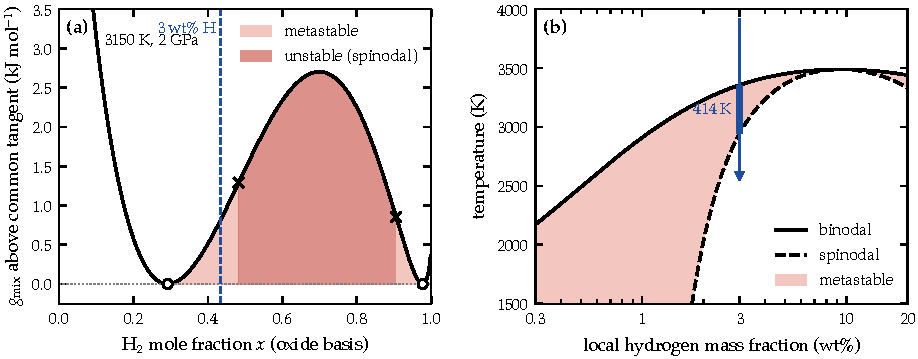
\includegraphics[width=\textwidth]{fig1_1_concept}
\thesiscaption{Binodal, spinodal and the metastable window of a cooling H$_2$--MgSiO$_3$
parcel.}{(a) Homogeneous Gibbs energy of mixing at 2\,GPa and 3150\,K above its common
tangent, for the published mixing model \cite{gilmore2026}. Circles mark the coexisting
compositions (binodal), crosses the inflection points (spinodal). A parcel with 3\,wt\%
local hydrogen (dashed line) is metastable here. (b) Binodal and spinodal temperatures at
2\,GPa as a function of local hydrogen mass fraction. A 3\,wt\% parcel cooling at fixed
pressure (arrow) enters the miscibility gap at the binodal but becomes unstable only at the
spinodal.}
\label{fig:concept}
\end{figure*}

The size of this window matters for sub-Neptunes, because it sets when, and at which
temperature, hydrogen leaves the interior. Delayed exsolution would release hydrogen later
and more abruptly. Through the atmospheric hydrogen budget, the timing of this release
feeds into the speciation equilibria that set the observable composition, such as the
H$_2$O/H$_2$ and CO$_2$/CH$_4$ ratios that we studied in our thesis \cite{laga2025}, and the
silane--methane competition proposed as a magma-ocean diagnostic \cite{hakim2026}. Whether
the window is large enough to matter has not been quantified.

The spinodal is a property of the homogeneous free energy inside the miscibility gap.
Simulations of coexisting phases constrain where the gap is, but not the free energy of the
homogeneous fluid within it. A spinodal derived from a fitted mixing model therefore
inherits the assumptions of its functional form. This makes \textbf{identifiability} the
central question of this work: how far do the existing data constrain the metastable free
energy, and with it the delay?

\section{Objectives and Scope}

This work investigates the thermodynamic limits on hydrogen exsolution from sub-Neptune
magma oceans using \Atm{}, a python-based modeling framework. We focus specifically on
closed H$_2$--MgSiO$_3$ parcels with local hydrogen mass fractions ranging from 0.1\% to 20\%,
at pressures of 2 to 10\,GPa, cooling through temperatures of 2,000 to 4,000\,K. These local
mass fractions describe the fluid at the magma-atmosphere boundary, not the hydrogen budget
of the whole planet.

The primary objectives of this work are to:
\begin{enumerate}
\item \textbf{Implement the final 2026 hydrogen--silicate mixing model} \cite{gilmore2026} in
\Atm{}, with a consistent conversion between the published oxide composition basis and the
native formula units of \Atm{}.
\item \textbf{Quantify the metastable window} between binodal and spinodal along cooling
paths, and the hydrogen inventory that delayed exsolution could withhold from separation.
\item \textbf{Audit the published fit against its source simulations}, and resolve the
mismatches that this audit reveals.
\item \textbf{Determine how well existing data constrain the metastable free energy}, by
recalibrating several smooth model classes against the same data, and identify the
simulations that would settle the question.
\end{enumerate}

This work is constrained to equilibrium thermodynamics and its local stability limits. We
acknowledge that real planets may exhibit nucleation on existing interfaces, finite cooling
rates, convective mixing and settling of the separated phases. We do not compute a
nucleation rate, a planetary radius or an atmospheric spectrum. However, establishing the
stability limits is essential: they bound the largest possible delay, define the boundary
conditions for kinetic models, and identify which measurements are needed before a kinetic
model can be trusted.
